% Created 2018-10-30 Tue 21:46
% Intended LaTeX compiler: pdflatex
\documentclass[presentation]{beamer}
\usepackage[utf8]{inputenc}
\usepackage[T1]{fontenc}
\usepackage{graphicx}
\usepackage{grffile}
\usepackage{longtable}
\usepackage{wrapfig}
\usepackage{rotating}
\usepackage[normalem]{ulem}
\usepackage{amsmath}
\usepackage{textcomp}
\usepackage{amssymb}
\usepackage{capt-of}
\usepackage{natbib}
\usepackage[linktocpage,pdfstartview=FitH,colorlinks,
linkcolor=blue,anchorcolor=blue,
citecolor=blue,filecolor=blue,menucolor=blue,urlcolor=blue]{hyperref}
\setbeamertemplate{frame footer}{\insertshortauthor}
\setbeamerfont{page number in head/foot}{size=\tiny}
\setbeamercolor{footline}{fg=gray}
\usepackage{amsmath}
\author{Florian Hollenbach}
\usepackage[english]{isodate}
\usepackage{amsmath,amsthm,amssymb,amsfonts}
\usetheme{metropolis}
\usecolortheme{}
\usefonttheme{}
\useinnertheme{}
\useoutertheme{}
\author{Florian Hollenbach}
\date{\today}
\title{Political Science 209 - Fall 2018}
\subtitle{Probability II}

\hypersetup{
 pdfauthor={Florian Hollenbach},
 pdftitle={Political Science 209 - Fall 2018},
 pdfkeywords={},
 pdfsubject={},
 pdfcreator={Emacs 25.3.1 (Org mode 9.1.14)}, 
 pdflang={English}}
\begin{document}

\maketitle

\begin{frame}[label={sec:org5e4d75c}]{Conditional Probability}
\begin{center}
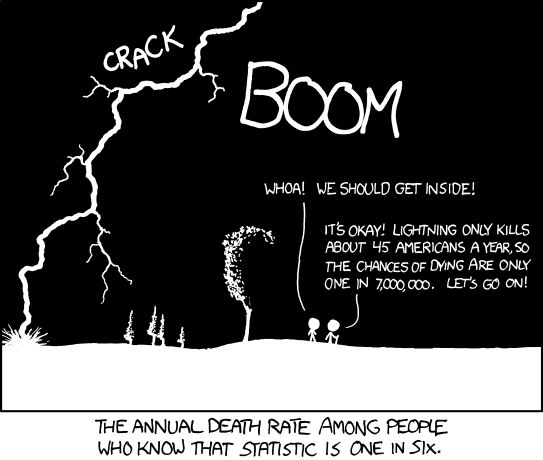
\includegraphics[width=8cm]{/Users/florianhollenbach/Documents/GitHub/Polisci209_2018/slides/week10/boom.png}
\end{center}
\end{frame}



\begin{frame}[label={sec:org4b0e454}]{Conditional Probability}
Sometimes information about one event can help inform us about likelihood of another event

Examples?

\pause

\begin{itemize}
\item What is the probability of rolling a 5 and then a 6?

\item What is the probability of rolling a 5 and then a 6 given that we rolled a 5 first?
\end{itemize}
\end{frame}

\begin{frame}[label={sec:orgaa6448e}]{Conditional Probability}
If it is cloudy outside, gives us additional information about likelihood of rain

If we know that one party will win the House, makes it more likely that party will win certain Senate races
\end{frame}

\begin{frame}[label={sec:org1109d85}]{Independence}
If the occurrence of one event (A) gives us information about likelihood of another event, then the two events are \alert{not} independent.

\pause

\alert{Independence} of two events implies that information about one event does not help us in knowing whether the second event will occur.
\end{frame}

\begin{frame}[label={sec:orgecbb0df}]{Independence}
For many real world examples, independence does not hold

Knowledge about other events allows us to improve guesses/probability calculations
\end{frame}

\begin{frame}[label={sec:orgcb5ed55}]{Conditional Probability}
P(A | B)

\emph{Probability of A given/conditional that B has happened}
\end{frame}

\begin{frame}[label={sec:org0cbece0}]{Conditional Probability}
P(A | B) = \(\frac{P(A and B)}{P(B)}\)


\emph{Probability of A and B happening (joint)  divided by probability of B happening (marginal)}
\end{frame}

\begin{frame}[label={sec:org592ef07}]{Conditional Probability}
Definitions:

P(A and B) - joint probability

P(A) - marginal probability
\end{frame}


\begin{frame}[label={sec:orgd7d7e54}]{Conditional Probability}
P(rolled 5 then 6) = ?

\pause

P(rolled 5 then 6) = \(\frac{1}{36}\)

P(rolled 5 then 6 | 5 first) =  \(\frac{P(5 then 6)}{P(5)}\)

\pause


\(\frac{\frac{1}{36}}{\frac{1}{6}} = \frac{1}{6}\)
\end{frame}


\begin{frame}[label={sec:orgdcc7201}]{Conditional Probability}
The probability that it is Friday and that a student is absent is 0.03. What is the probability that student is absent, given that it is Friday?

P(absent | Friday) = ?

\pause

P(absent | Friday) = \(\frac{0.03}{0.2} = 0.15\)
\end{frame}


\begin{frame}[label={sec:orgde5b536}]{Conditional Probability}
P(A | B) = \(\frac{P(A and B)}{P(B)}\)


Also means:

P(A and B) = P(A | B) P(B)
\end{frame}



\begin{frame}[label={sec:org8470792}]{Probability Problems}
What is the probability of drawing any card between 2 and
10, or jack, queen, king in any color?
\end{frame}


\begin{frame}[label={sec:orga5c984c}]{Probability Problems}
What is the probability of drawing two kings from a full deck of cards?

\pause

P(2 kings) = \(\frac{4}{52} \times\)?

\pause

P(2 kings) = \(\frac{4}{52} \times \frac{3}{51} = \frac{12}{2652} =\frac{1}{221}\)
\end{frame}


\begin{frame}[label={sec:org4501153}]{Probability Problems}
\begin{center}
\begin{tabular}{lrrr}
Annual income & Took 209 & Took 309 & TOTAL\\
Under \$50,000 & 30 & 5 & 35\\
\$50,000 to \$100,000 & 25 & 6 & 35\\
over \$100,000 & 10 & 9 & 19\\
\end{tabular}
\end{center}

What is the probability of any student making over \$100,000?
\end{frame}



\begin{frame}[label={sec:org2cab0ff}]{Probability Problems}
\begin{center}
\begin{tabular}{lrrr}
Annual income & Took 209 & Took 309 & TOTAL\\
Under \$50,000 & 30 & 5 & 35\\
\$50,000 to \$100,000 & 25 & 6 & 35\\
over \$100,000 & 10 & 9 & 19\\
\end{tabular}
\end{center}

What is the probability of a student making over \$100,000, conditional that he took 309?
\end{frame}



\begin{frame}[label={sec:org80a4179}]{Probability Problems}
\begin{center}
\begin{tabular}{lrrr}
Annual income & Took 209 & Took 309 & TOTAL\\
Under \$50,000 & 30 & 5 & 35\\
\$50,000 to \$100,000 & 25 & 6 & 35\\
over \$100,000 & 10 & 9 & 19\\
\end{tabular}
\end{center}


What is the probability of a having taken 309, conditional on  making over \$100,000?
\end{frame}
\end{document}